\documentclass[]{article}
\usepackage{lmodern}
\usepackage{amssymb,amsmath}
\usepackage{ifxetex,ifluatex}
\usepackage{fixltx2e} % provides \textsubscript
\ifnum 0\ifxetex 1\fi\ifluatex 1\fi=0 % if pdftex
  \usepackage[T1]{fontenc}
  \usepackage[utf8]{inputenc}
\else % if luatex or xelatex
  \ifxetex
    \usepackage{mathspec}
    \usepackage{xltxtra,xunicode}
  \else
    \usepackage{fontspec}
  \fi
  \defaultfontfeatures{Mapping=tex-text,Scale=MatchLowercase}
  \newcommand{\euro}{€}
\fi
% use upquote if available, for straight quotes in verbatim environments
\IfFileExists{upquote.sty}{\usepackage{upquote}}{}
% use microtype if available
\IfFileExists{microtype.sty}{%
\usepackage{microtype}
\UseMicrotypeSet[protrusion]{basicmath} % disable protrusion for tt fonts
}{}
\usepackage[margin=1in]{geometry}
\usepackage{color}
\usepackage{fancyvrb}
\newcommand{\VerbBar}{|}
\newcommand{\VERB}{\Verb[commandchars=\\\{\}]}
\DefineVerbatimEnvironment{Highlighting}{Verbatim}{commandchars=\\\{\}}
% Add ',fontsize=\small' for more characters per line
\usepackage{framed}
\definecolor{shadecolor}{RGB}{248,248,248}
\newenvironment{Shaded}{\begin{snugshade}}{\end{snugshade}}
\newcommand{\KeywordTok}[1]{\textcolor[rgb]{0.13,0.29,0.53}{\textbf{{#1}}}}
\newcommand{\DataTypeTok}[1]{\textcolor[rgb]{0.13,0.29,0.53}{{#1}}}
\newcommand{\DecValTok}[1]{\textcolor[rgb]{0.00,0.00,0.81}{{#1}}}
\newcommand{\BaseNTok}[1]{\textcolor[rgb]{0.00,0.00,0.81}{{#1}}}
\newcommand{\FloatTok}[1]{\textcolor[rgb]{0.00,0.00,0.81}{{#1}}}
\newcommand{\CharTok}[1]{\textcolor[rgb]{0.31,0.60,0.02}{{#1}}}
\newcommand{\StringTok}[1]{\textcolor[rgb]{0.31,0.60,0.02}{{#1}}}
\newcommand{\CommentTok}[1]{\textcolor[rgb]{0.56,0.35,0.01}{\textit{{#1}}}}
\newcommand{\OtherTok}[1]{\textcolor[rgb]{0.56,0.35,0.01}{{#1}}}
\newcommand{\AlertTok}[1]{\textcolor[rgb]{0.94,0.16,0.16}{{#1}}}
\newcommand{\FunctionTok}[1]{\textcolor[rgb]{0.00,0.00,0.00}{{#1}}}
\newcommand{\RegionMarkerTok}[1]{{#1}}
\newcommand{\ErrorTok}[1]{\textbf{{#1}}}
\newcommand{\NormalTok}[1]{{#1}}
\usepackage{graphicx}
\makeatletter
\def\maxwidth{\ifdim\Gin@nat@width>\linewidth\linewidth\else\Gin@nat@width\fi}
\def\maxheight{\ifdim\Gin@nat@height>\textheight\textheight\else\Gin@nat@height\fi}
\makeatother
% Scale images if necessary, so that they will not overflow the page
% margins by default, and it is still possible to overwrite the defaults
% using explicit options in \includegraphics[width, height, ...]{}
\setkeys{Gin}{width=\maxwidth,height=\maxheight,keepaspectratio}
\ifxetex
  \usepackage[setpagesize=false, % page size defined by xetex
              unicode=false, % unicode breaks when used with xetex
              xetex]{hyperref}
\else
  \usepackage[unicode=true]{hyperref}
\fi
\hypersetup{breaklinks=true,
            bookmarks=true,
            pdfauthor={},
            pdftitle={Vectorización, la familia apply y otros},
            colorlinks=true,
            citecolor=blue,
            urlcolor=blue,
            linkcolor=magenta,
            pdfborder={0 0 0}}
\urlstyle{same}  % don't use monospace font for urls
\setlength{\parindent}{0pt}
\setlength{\parskip}{6pt plus 2pt minus 1pt}
\setlength{\emergencystretch}{3em}  % prevent overfull lines
\setcounter{secnumdepth}{0}

%%% Use protect on footnotes to avoid problems with footnotes in titles
\let\rmarkdownfootnote\footnote%
\def\footnote{\protect\rmarkdownfootnote}

%%% Change title format to be more compact
\usepackage{titling}

% Create subtitle command for use in maketitle
\newcommand{\subtitle}[1]{
  \posttitle{
    \begin{center}\large#1\end{center}
    }
}

\setlength{\droptitle}{-2em}
  \title{Vectorización, la familia apply y otros}
  \pretitle{\vspace{\droptitle}\centering\huge}
  \posttitle{\par}
  \author{}
  \preauthor{}\postauthor{}
  \date{}
  \predate{}\postdate{}

\usepackage[
  backend=biber,
  style=alphabetic,
  sorting=ynt,
  citestyle=authoryear
  ]{biblatex}
\addbibresource{../lit/bib.bib}

\usepackage[utf8]{inputenc}
\usepackage[spanish]{babel}

%%%% Frames
\ifxetex
    \makeatletter % undo the wrong changes made by mathspec
    \let\RequirePackage\original@RequirePackage
    \let\usepackage\RequirePackage
    \makeatother
\fi

\usepackage{xcolor}
\usepackage[tikz]{bclogo}
\usepackage[framemethod=tikz]{mdframed}
\usepackage{lipsum}
\usepackage[many]{tcolorbox}

\definecolor{bgblue}{RGB}{245,243,253}
\definecolor{ttblue}{RGB}{91,194,224}
\definecolor{llred}{RGB}{255,228,225}
\definecolor{bbblack}{RGB}{0,0,0}

\mdfdefinestyle{mystyle}{%
  rightline=true,
  innerleftmargin=10,
  innerrightmargin=10,
  outerlinewidth=3pt,
  topline=false,
  rightline=true,
  bottomline=false,
  skipabove=\topsep,
  skipbelow=\topsep
}

\newtcolorbox{curiosidad}[1][]{
  breakable,
  title=#1,
  colback=white,
  colbacktitle=white,
  coltitle=black,
  fonttitle=\bfseries,
  bottomrule=0pt,
  toprule=0pt,
  leftrule=3pt,
  rightrule=3pt,
  titlerule=0pt,
  arc=0pt,
  outer arc=0pt,
  colframe=black,
}

\newtcolorbox{nota}[1][]{
  breakable,
  freelance,
  title=#1,
  colback=white,
  colbacktitle=white,
  coltitle=black,
  fonttitle=\bfseries,
  bottomrule=0pt,
  boxrule=0pt,
  colframe=white,
  overlay unbroken and first={
  \draw[red!75!black,line width=3pt]
    ([xshift=5pt]frame.north west) -- 
    (frame.north west) -- 
    (frame.south west);
  \draw[red!75!black,line width=3pt]
    ([xshift=-5pt]frame.north east) -- 
    (frame.north east) -- 
    (frame.south east);
  },
  overlay unbroken app={
  \draw[red!75!black,line width=3pt,line cap=rect]
    (frame.south west) -- 
    ([xshift=5pt]frame.south west);
  \draw[red!75!black,line width=3pt,line cap=rect]
    (frame.south east) -- 
    ([xshift=-5pt]frame.south east);
  },
  overlay middle and last={
  \draw[red!75!black,line width=3pt]
    (frame.north west) -- 
    (frame.south west);
  \draw[red!75!black,line width=3pt]
    (frame.north east) -- 
    (frame.south east);
  },
  overlay last app={
  \draw[red!75!black,line width=3pt,line cap=rect]
    (frame.south west) --
    ([xshift=5pt]frame.south west);
  \draw[red!75!black,line width=3pt,line cap=rect]
    (frame.south east) --
    ([xshift=-5pt]frame.south east);
  },
}


\begin{document}

\maketitle


\section{Subconjuntos de diferentes estructuras de
datos}\label{subconjuntos-de-diferentes-estructuras-de-datos}

Esta sección está basada en \textcite[Subsetting]{wickham2014advanced}
disponible en
\href{http://adv-r.had.co.nz/Subsetting.html\#subsetting-operators}{línea}.

Aprender a extraer subconjuntos de los datos es importante y permite
realizar operaciones complejas con los mismos. De los conceptos
importantes que se deben aprender son

\begin{itemize}
\itemsep1pt\parskip0pt\parsep0pt
\item
  Los operadores para extraer subconjuntos (subsetting operators)
\item
  Los 6 tipos de extracciones de subconjuntos
\item
  Las diferencias a la hora de extraer subconjuntos de las diferentes
  estructuras de datos (factores, listas, matrices, dataframes)
\item
  El uso de la extracción de subconjuntos junto a asignar variables.
\end{itemize}

Cuando tenemos que extraer pedazos de los datos (o analizar solamente
parte de éstos), necesitamos complementar \texttt{str()} con
\texttt{{[}{[}}, es decir, la estructura nos dirá cómo utilizar el
operador subconjunto de manera que de hecho extraigamos lo que queremos.

\subsection{Operadores para extraer
subconjuntos}\label{operadores-para-extraer-subconjuntos}

Dependiendo la estructura de datos que tenemos, será la forma en la que
extraemos elementos de ella. Hay dos operadores de subconjunto:
\texttt{{[}{[}} y \texttt{\$}. \texttt{{[}{[}} se parece a \texttt{{[}}
pero regresa un solo valor y te permite sacar pedazos de una lista.
\texttt{\$} es un atajo útil para \texttt{{[}{[}}.

\subsubsection{Vectores atómicos}\label{vectores-atomicos}

¿De qué formas puedo extraer elementos de un vector? Hay varias maneras
\textbf{sin importar} la \emph{clase} del vector.

\begin{itemize}
\itemsep1pt\parskip0pt\parsep0pt
\item
  \textbf{Enteros positivos} regresan los elementos en las posiciones
  especificadas en el orden que especificamos.
\end{itemize}

\begin{Shaded}
\begin{Highlighting}[]
\NormalTok{x <-}\StringTok{ }\KeywordTok{c}\NormalTok{(}\FloatTok{5.6}\NormalTok{, }\FloatTok{7.8}\NormalTok{, }\FloatTok{4.5}\NormalTok{, }\FloatTok{3.3}\NormalTok{)}

\NormalTok{x[}\KeywordTok{c}\NormalTok{(}\DecValTok{3}\NormalTok{, }\DecValTok{1}\NormalTok{)]}
\end{Highlighting}
\end{Shaded}

\begin{verbatim}
## [1] 4.5 5.6
\end{verbatim}

\begin{Shaded}
\begin{Highlighting}[]
\NormalTok{## Si duplicamos posiciones, nos regresa resultados duplicados}
\NormalTok{x[}\KeywordTok{c}\NormalTok{(}\DecValTok{1}\NormalTok{, }\DecValTok{1}\NormalTok{, }\DecValTok{1}\NormalTok{)]}
\end{Highlighting}
\end{Shaded}

\begin{verbatim}
## [1] 5.6 5.6 5.6
\end{verbatim}

\begin{Shaded}
\begin{Highlighting}[]
\NormalTok{## Si usamos valores reales, se coerciona a entero}
\NormalTok{x[}\KeywordTok{c}\NormalTok{(}\FloatTok{1.1}\NormalTok{, }\FloatTok{2.4}\NormalTok{)]}
\end{Highlighting}
\end{Shaded}

\begin{verbatim}
## [1] 5.6 7.8
\end{verbatim}

\begin{Shaded}
\begin{Highlighting}[]
\NormalTok{x[}\KeywordTok{order}\NormalTok{(x)]}
\end{Highlighting}
\end{Shaded}

\begin{verbatim}
## [1] 3.3 4.5 5.6 7.8
\end{verbatim}

\begin{Shaded}
\begin{Highlighting}[]
\NormalTok{x[}\KeywordTok{order}\NormalTok{(x, }\DataTypeTok{decreasing =} \NormalTok{T)]}
\end{Highlighting}
\end{Shaded}

\begin{verbatim}
## [1] 7.8 5.6 4.5 3.3
\end{verbatim}

\begin{itemize}
\itemsep1pt\parskip0pt\parsep0pt
\item
  \textbf{Enteros negativos} omiten los valores en las posiciones que se
  especifican.
\end{itemize}

\begin{Shaded}
\begin{Highlighting}[]
\NormalTok{x}
\end{Highlighting}
\end{Shaded}

\begin{verbatim}
## [1] 5.6 7.8 4.5 3.3
\end{verbatim}

\begin{Shaded}
\begin{Highlighting}[]
\NormalTok{x[-}\KeywordTok{c}\NormalTok{(}\DecValTok{3}\NormalTok{, }\DecValTok{1}\NormalTok{)]}
\end{Highlighting}
\end{Shaded}

\begin{verbatim}
## [1] 7.8 3.3
\end{verbatim}

\emph{Mezclar} no funciona.

\begin{Shaded}
\begin{Highlighting}[]
\NormalTok{x[}\KeywordTok{c}\NormalTok{(-}\DecValTok{3}\NormalTok{, }\DecValTok{1}\NormalTok{)]}
\end{Highlighting}
\end{Shaded}

\begin{itemize}
\itemsep1pt\parskip0pt\parsep0pt
\item
  \textbf{Vectores lógicos} selecciona los elementos cuyo valor
  correspondiente es \texttt{TRUE}. Esta es una de los tipos más útiles.
\end{itemize}

\begin{Shaded}
\begin{Highlighting}[]
\NormalTok{x[}\KeywordTok{c}\NormalTok{(}\OtherTok{TRUE}\NormalTok{, }\OtherTok{TRUE}\NormalTok{, }\OtherTok{FALSE}\NormalTok{, }\OtherTok{FALSE}\NormalTok{)]}
\end{Highlighting}
\end{Shaded}

\begin{verbatim}
## [1] 5.6 7.8
\end{verbatim}

\begin{Shaded}
\begin{Highlighting}[]
\NormalTok{x[c(}\OtherTok{TRUE}\NormalTok{, }\OtherTok{FALSE}\ErrorTok{)}\NormalTok{] }\CommentTok{# Autocompleta el vector lógico al tamaño de x}
\end{Highlighting}
\end{Shaded}

\begin{verbatim}
## [1] 5.6 4.5
\end{verbatim}

\begin{Shaded}
\begin{Highlighting}[]
\NormalTok{x[}\KeywordTok{c}\NormalTok{(}\OtherTok{TRUE}\NormalTok{, }\OtherTok{TRUE}\NormalTok{, }\OtherTok{NA}\NormalTok{, }\OtherTok{FALSE}\NormalTok{)]}
\end{Highlighting}
\end{Shaded}

\begin{verbatim}
## [1] 5.6 7.8  NA
\end{verbatim}

\begin{itemize}
\itemsep1pt\parskip0pt\parsep0pt
\item
  \textbf{Nada} si no especifico nada, me regresa el vector original
\end{itemize}

\begin{Shaded}
\begin{Highlighting}[]
\NormalTok{x[]}
\end{Highlighting}
\end{Shaded}

\begin{verbatim}
## [1] 5.6 7.8 4.5 3.3
\end{verbatim}

\begin{itemize}
\itemsep1pt\parskip0pt\parsep0pt
\item
  \textbf{Cero} el índice cero no aplica en R, te regresa el vector
  vacio
\end{itemize}

\begin{Shaded}
\begin{Highlighting}[]
\NormalTok{x[}\DecValTok{0}\NormalTok{]}
\end{Highlighting}
\end{Shaded}

\begin{verbatim}
## numeric(0)
\end{verbatim}

\begin{itemize}
\itemsep1pt\parskip0pt\parsep0pt
\item
  Si el vector tiene \textbf{nombres} también los puedo usar.
\end{itemize}

\begin{Shaded}
\begin{Highlighting}[]
\KeywordTok{names}\NormalTok{(x) <-}\StringTok{ }\KeywordTok{c}\NormalTok{(}\StringTok{"a"}\NormalTok{, }\StringTok{"ab"}\NormalTok{, }\StringTok{"b"}\NormalTok{, }\StringTok{"c"}\NormalTok{)}
\NormalTok{x[}\StringTok{"ab"}\NormalTok{]}
\end{Highlighting}
\end{Shaded}

\begin{verbatim}
##  ab 
## 7.8
\end{verbatim}

\begin{Shaded}
\begin{Highlighting}[]
\NormalTok{x[}\StringTok{"d"}\NormalTok{]}
\end{Highlighting}
\end{Shaded}

\begin{verbatim}
## <NA> 
##   NA
\end{verbatim}

\begin{Shaded}
\begin{Highlighting}[]
\NormalTok{x[}\KeywordTok{grep}\NormalTok{(}\StringTok{"a"}\NormalTok{, }\KeywordTok{names}\NormalTok{(x))]}
\end{Highlighting}
\end{Shaded}

\begin{verbatim}
##   a  ab 
## 5.6 7.8
\end{verbatim}

Las \textbf{listas} operan básicamente igual a vectores recordando que
si usamos \texttt{{[}} regresa una lista y tanto \texttt{{[}{[}} y
\texttt{\$} extrae componentes de la lista.

\subsubsection{Matrices y arreglos}\label{matrices-y-arreglos}

Para estructuras de mayor dimensión se pueden extraer de tres maneras:

\begin{itemize}
\itemsep1pt\parskip0pt\parsep0pt
\item
  Con vectores múltiples
\item
  Con un solo vector
\item
  Con una matriz
\end{itemize}

\begin{Shaded}
\begin{Highlighting}[]
\NormalTok{m <-}\StringTok{ }\KeywordTok{matrix}\NormalTok{(}\DecValTok{1}\NormalTok{:}\DecValTok{12}\NormalTok{, }\DataTypeTok{nrow =} \DecValTok{3}\NormalTok{)}
\KeywordTok{colnames}\NormalTok{(m) <-}\StringTok{ }\NormalTok{LETTERS[}\DecValTok{1}\NormalTok{:}\DecValTok{4}\NormalTok{]}
\NormalTok{m[}\DecValTok{1}\NormalTok{:}\DecValTok{2}\NormalTok{, ]}
\end{Highlighting}
\end{Shaded}

\begin{verbatim}
##      A B C  D
## [1,] 1 4 7 10
## [2,] 2 5 8 11
\end{verbatim}

\begin{Shaded}
\begin{Highlighting}[]
\NormalTok{m[}\KeywordTok{c}\NormalTok{(T, F, F), }\KeywordTok{c}\NormalTok{(}\StringTok{"B"}\NormalTok{, }\StringTok{"C"}\NormalTok{)]}
\end{Highlighting}
\end{Shaded}

\begin{verbatim}
## B C 
## 4 7
\end{verbatim}

\begin{Shaded}
\begin{Highlighting}[]
\NormalTok{m[}\DecValTok{1}\NormalTok{, }\DecValTok{4}\NormalTok{]}
\end{Highlighting}
\end{Shaded}

\begin{verbatim}
##  D 
## 10
\end{verbatim}

Como ven, es solamente generalizar lo que se hace en vectores
replicándolo al número de dimensiones que se tiene.

\begin{Shaded}
\begin{Highlighting}[]
\NormalTok{m[}\KeywordTok{c}\NormalTok{(T, F, F)]}
\end{Highlighting}
\end{Shaded}

\begin{verbatim}
## [1]  1  4  7 10
\end{verbatim}

\begin{Shaded}
\begin{Highlighting}[]
\KeywordTok{class}\NormalTok{(m[}\KeywordTok{c}\NormalTok{(T, F, F)])}
\end{Highlighting}
\end{Shaded}

\begin{verbatim}
## [1] "integer"
\end{verbatim}

\texttt{{[}} simplifica al objeto. En matriz, me quita la
dimensionalidad, en listas me da lo que esta dentro de esa celda.

\subsubsection{Dataframes}\label{dataframes}

\begin{Shaded}
\begin{Highlighting}[]
\NormalTok{df <-}\StringTok{ }\KeywordTok{data.frame}\NormalTok{(}\DataTypeTok{x =} \DecValTok{1}\NormalTok{:}\DecValTok{3}\NormalTok{, }\DataTypeTok{y =} \DecValTok{3}\NormalTok{:}\DecValTok{1}\NormalTok{, }\DataTypeTok{z =} \NormalTok{letters[}\DecValTok{1}\NormalTok{:}\DecValTok{3}\NormalTok{])}

\NormalTok{df[}\KeywordTok{c}\NormalTok{(}\DecValTok{1}\NormalTok{, }\DecValTok{2}\NormalTok{), ]}
\end{Highlighting}
\end{Shaded}

\begin{verbatim}
##   x y z
## 1 1 3 a
## 2 2 2 b
\end{verbatim}

\begin{Shaded}
\begin{Highlighting}[]
\NormalTok{df[, }\KeywordTok{c}\NormalTok{(}\DecValTok{1}\NormalTok{, }\DecValTok{2}\NormalTok{)]}
\end{Highlighting}
\end{Shaded}

\begin{verbatim}
##   x y
## 1 1 3
## 2 2 2
## 3 3 1
\end{verbatim}

\begin{Shaded}
\begin{Highlighting}[]
\NormalTok{df[, }\KeywordTok{c}\NormalTok{(}\StringTok{"z"}\NormalTok{, }\StringTok{"x"}\NormalTok{)]}
\end{Highlighting}
\end{Shaded}

\begin{verbatim}
##   z x
## 1 a 1
## 2 b 2
## 3 c 3
\end{verbatim}

\begin{Shaded}
\begin{Highlighting}[]
\NormalTok{df[}\KeywordTok{c}\NormalTok{(}\StringTok{"z"}\NormalTok{, }\StringTok{"x"}\NormalTok{)]}
\end{Highlighting}
\end{Shaded}

\begin{verbatim}
##   z x
## 1 a 1
## 2 b 2
## 3 c 3
\end{verbatim}

\begin{Shaded}
\begin{Highlighting}[]
\KeywordTok{class}\NormalTok{(df[, }\KeywordTok{c}\NormalTok{(}\StringTok{"z"}\NormalTok{, }\StringTok{"x"}\NormalTok{)])}
\end{Highlighting}
\end{Shaded}

\begin{verbatim}
## [1] "data.frame"
\end{verbatim}

\begin{Shaded}
\begin{Highlighting}[]
\KeywordTok{class}\NormalTok{(df[}\KeywordTok{c}\NormalTok{(}\StringTok{"z"}\NormalTok{, }\StringTok{"x"}\NormalTok{)])}
\end{Highlighting}
\end{Shaded}

\begin{verbatim}
## [1] "data.frame"
\end{verbatim}

\begin{Shaded}
\begin{Highlighting}[]
\KeywordTok{str}\NormalTok{(df[}\StringTok{"x"}\NormalTok{])}
\end{Highlighting}
\end{Shaded}

\begin{verbatim}
## 'data.frame':    3 obs. of  1 variable:
##  $ x: int  1 2 3
\end{verbatim}

\begin{Shaded}
\begin{Highlighting}[]
\KeywordTok{str}\NormalTok{(df[, }\StringTok{"x"}\NormalTok{])}
\end{Highlighting}
\end{Shaded}

\begin{verbatim}
##  int [1:3] 1 2 3
\end{verbatim}

\begin{Shaded}
\begin{Highlighting}[]
\KeywordTok{str}\NormalTok{(df$x)}
\end{Highlighting}
\end{Shaded}

\begin{verbatim}
##  int [1:3] 1 2 3
\end{verbatim}

\renewcommand\bcStyleTitre[1]{\large\textcolor{bbblack}{#1}}

\begin{bclogo}[
  couleur=llred,
  arrondi=0,
  logo=\bcstop,
  barre=none,
  noborder=true]{Ejercicios}
\begin{enumerate}
\item Utiliza la base mtcars
\item{Arregla los errores al extraer subconjuntos en dataframes
\begin{verbatim}
mtcars[mtcars$cyl = 4, ]
mtcars[-1:4, ]
mtcars[mtcars$cyl <= 5]
mtcars[mtcars$cyl == 4 | 6, ]
\end{verbatim}
}
\item ¿Por qué al correr {\it x <- 1:5; x[NA] } obtengo valores perdidos?
\item Genera una matriz cuadrada tamaño 5 llamada m. ¿Qué te da correr m[upper.tri(m)]?
\item ¿Por qué al realizar mtcars[1:20] me da un error? ¿Por qué mtcars[1:2] no me lo da?
¿Por qué mtcars[1:20, ] es distinto?
\item Haz una función que extraiga la diagonal de la matriz m que creaste antes.
Debe dar el mismo resultado que ejecutar diag(m)
\item ¿Qué hace df[is.na(df)] <- 0?
\end{enumerate}
\end{bclogo}

\subsection{Asignar a un subconjunto}\label{asignar-a-un-subconjunto}

Muchas veces lo que necesitamos es encontrar ciertos valores para poder
reemplazarlos con algo más. Por ejemplo, muchas veces queremos imputar
valores perdidos con cierto valor.

\begin{Shaded}
\begin{Highlighting}[]
\CommentTok{# Variables continuas}
\NormalTok{x <-}\StringTok{ }\KeywordTok{c}\NormalTok{(}\DecValTok{1}\NormalTok{, }\DecValTok{2}\NormalTok{, }\DecValTok{3}\NormalTok{, }\OtherTok{NA}\NormalTok{, }\OtherTok{NaN}\NormalTok{, }\DecValTok{7}\NormalTok{)}
\NormalTok{media <-}\StringTok{ }\KeywordTok{mean}\NormalTok{(x, }\DataTypeTok{na.rm =} \NormalTok{T)}
\NormalTok{media}
\end{Highlighting}
\end{Shaded}

\begin{verbatim}
## [1] 3.25
\end{verbatim}

\begin{Shaded}
\begin{Highlighting}[]
\NormalTok{x[}\KeywordTok{is.na}\NormalTok{(x)] <-}\StringTok{ }\NormalTok{media}
\NormalTok{x}
\end{Highlighting}
\end{Shaded}

\begin{verbatim}
## [1] 1.00 2.00 3.00 3.25 3.25 7.00
\end{verbatim}

\begin{Shaded}
\begin{Highlighting}[]
\CommentTok{# Variables discretas}
\NormalTok{x <-}\StringTok{ }\KeywordTok{c}\NormalTok{(}\KeywordTok{rep}\NormalTok{(}\StringTok{"azul"}\NormalTok{, }\DecValTok{3}\NormalTok{), }\StringTok{"verde"}\NormalTok{, }\OtherTok{NA}\NormalTok{, }\StringTok{"verde"}\NormalTok{, }\KeywordTok{rep}\NormalTok{(}\StringTok{"rojo"}\NormalTok{, }\DecValTok{4}\NormalTok{))}
\NormalTok{x}
\end{Highlighting}
\end{Shaded}

\begin{verbatim}
##  [1] "azul"  "azul"  "azul"  "verde" NA      "verde" "rojo"  "rojo" 
##  [9] "rojo"  "rojo"
\end{verbatim}

\begin{Shaded}
\begin{Highlighting}[]
\NormalTok{moda <-}\StringTok{ }\KeywordTok{names}\NormalTok{(}\KeywordTok{table}\NormalTok{(x))[}\KeywordTok{which}\NormalTok{(}\KeywordTok{table}\NormalTok{(x) ==}\StringTok{ }\KeywordTok{max}\NormalTok{(}\KeywordTok{table}\NormalTok{(x)))] }\CommentTok{# Engorroso, no?}
\NormalTok{x[}\KeywordTok{is.na}\NormalTok{(x)] <-}\StringTok{ }\NormalTok{moda}
\NormalTok{x}
\end{Highlighting}
\end{Shaded}

\begin{verbatim}
##  [1] "azul"  "azul"  "azul"  "verde" "rojo"  "verde" "rojo"  "rojo" 
##  [9] "rojo"  "rojo"
\end{verbatim}

\begin{Shaded}
\begin{Highlighting}[]
\CommentTok{# Puedo reemplazar partes de un vector}
\NormalTok{x <-}\StringTok{ }\DecValTok{1}\NormalTok{:}\DecValTok{5}
\NormalTok{x[}\KeywordTok{c}\NormalTok{(}\DecValTok{1}\NormalTok{, }\DecValTok{2}\NormalTok{)] <-}\StringTok{ }\DecValTok{2}\NormalTok{:}\DecValTok{3}
\NormalTok{x}
\end{Highlighting}
\end{Shaded}

\begin{verbatim}
## [1] 2 3 3 4 5
\end{verbatim}

\begin{Shaded}
\begin{Highlighting}[]
\CommentTok{# Las longitudes de las asignaciones tienen que ser iguales}
\NormalTok{x[-}\DecValTok{1}\NormalTok{] <-}\StringTok{ }\DecValTok{4}\NormalTok{:}\DecValTok{1}
\NormalTok{x}
\end{Highlighting}
\end{Shaded}

\begin{verbatim}
## [1] 2 4 3 2 1
\end{verbatim}

\begin{Shaded}
\begin{Highlighting}[]
\CommentTok{# No se revisan duplicados}
\NormalTok{x[}\KeywordTok{c}\NormalTok{(}\DecValTok{1}\NormalTok{, }\DecValTok{1}\NormalTok{)] <-}\StringTok{ }\DecValTok{2}\NormalTok{:}\DecValTok{3}
\NormalTok{x}
\end{Highlighting}
\end{Shaded}

\begin{verbatim}
## [1] 3 4 3 2 1
\end{verbatim}

\begin{Shaded}
\begin{Highlighting}[]
\CommentTok{# Puedo sustituir valores considerando toda la logica }
\NormalTok{x <-}\StringTok{ }\KeywordTok{c}\NormalTok{(}\DecValTok{1}\NormalTok{:}\DecValTok{10}\NormalTok{)}
\NormalTok{x[x >}\StringTok{ }\DecValTok{5}\NormalTok{] <-}\StringTok{ }\DecValTok{0}
\NormalTok{x}
\end{Highlighting}
\end{Shaded}

\begin{verbatim}
##  [1] 1 2 3 4 5 0 0 0 0 0
\end{verbatim}

Por último, es útil notar la utilidad de asignar utilizando la forma de
asignar \textbf{nada} mencionada anteriormente.

\begin{Shaded}
\begin{Highlighting}[]
\KeywordTok{class}\NormalTok{(mtcars)}
\end{Highlighting}
\end{Shaded}

\begin{verbatim}
## [1] "data.frame"
\end{verbatim}

\begin{Shaded}
\begin{Highlighting}[]
\NormalTok{mtcars[] <-}\StringTok{ }\KeywordTok{lapply}\NormalTok{(mtcars, as.integer)}
\KeywordTok{class}\NormalTok{(mtcars)}
\end{Highlighting}
\end{Shaded}

\begin{verbatim}
## [1] "data.frame"
\end{verbatim}

\begin{Shaded}
\begin{Highlighting}[]
\KeywordTok{dim}\NormalTok{(mtcars)}
\end{Highlighting}
\end{Shaded}

\begin{verbatim}
## [1] 32 11
\end{verbatim}

\begin{Shaded}
\begin{Highlighting}[]
\NormalTok{mtcars <-}\StringTok{ }\KeywordTok{lapply}\NormalTok{(mtcars, as.integer)}
\KeywordTok{class}\NormalTok{(mtcars)}
\end{Highlighting}
\end{Shaded}

\begin{verbatim}
## [1] "list"
\end{verbatim}

\begin{Shaded}
\begin{Highlighting}[]
\KeywordTok{dim}\NormalTok{(mtcars)}
\end{Highlighting}
\end{Shaded}

\begin{verbatim}
## NULL
\end{verbatim}

Asignar utilizando el operador de suconjunto a nada nos permite
preservar la estructura del objeto original así como su clase.

En el caso de listas, si combinamos un operador de sunjunto mas
asignación a nulo, podemos remover objetos de ésta.

\begin{Shaded}
\begin{Highlighting}[]
\NormalTok{x <-}\StringTok{ }\KeywordTok{list}\NormalTok{(}\DataTypeTok{a =} \DecValTok{1}\NormalTok{, }\DataTypeTok{b =} \DecValTok{2}\NormalTok{)}
\NormalTok{x[[}\DecValTok{2}\NormalTok{]] <-}\StringTok{ }\OtherTok{NULL}
\KeywordTok{str}\NormalTok{(x)}
\end{Highlighting}
\end{Shaded}

\begin{verbatim}
## List of 1
##  $ a: num 1
\end{verbatim}

\begin{Shaded}
\begin{Highlighting}[]
\NormalTok{x[}\StringTok{"b"}\NormalTok{] <-}\StringTok{ }\KeywordTok{list}\NormalTok{(}\OtherTok{NULL}\NormalTok{)}
\KeywordTok{str}\NormalTok{(x)}
\end{Highlighting}
\end{Shaded}

\begin{verbatim}
## List of 2
##  $ a: num 1
##  $ b: NULL
\end{verbatim}

\subsection{Operadores lógicos}\label{operadores-logicos}

\begin{table}[ht]
\centering
\begin{tabular}{ll}
  \hline
Operador & Descripción \\ 
  \hline
$<$ & menor que \\ 
  $<$= & menor o igual que \\ 
  $>$ & mayor que \\ 
  == & exactamente igual que \\ 
  != & diferente de \\ 
  !x &  no x \\ 
  x $|$ y & x O y \\ 
  x \& y & x Y y \\ 
  isTRUE(x) & checa si x es verdadero \\ 
   \hline
\end{tabular}
\end{table}

\textbf{Ejemplo}: Supongamos que queremos saber qué elementos de $x$ son
menores que $5$ y mayores que $8$.

\begin{Shaded}
\begin{Highlighting}[]
\NormalTok{x <-}\StringTok{ }\KeywordTok{c}\NormalTok{(}\DecValTok{1}\NormalTok{:}\DecValTok{10}\NormalTok{)}
\NormalTok{x[(x>}\DecValTok{8}\NormalTok{) |}\StringTok{ }\NormalTok{(x<}\DecValTok{5}\NormalTok{)]}
\end{Highlighting}
\end{Shaded}

\begin{verbatim}
## [1]  1  2  3  4  9 10
\end{verbatim}

\begin{Shaded}
\begin{Highlighting}[]
\CommentTok{# ¿Cómo funciona?}
\NormalTok{x}
\end{Highlighting}
\end{Shaded}

\begin{verbatim}
##  [1]  1  2  3  4  5  6  7  8  9 10
\end{verbatim}

\begin{Shaded}
\begin{Highlighting}[]
\NormalTok{x >}\StringTok{ }\DecValTok{8}
\end{Highlighting}
\end{Shaded}

\begin{verbatim}
##  [1] FALSE FALSE FALSE FALSE FALSE FALSE FALSE FALSE  TRUE  TRUE
\end{verbatim}

\begin{Shaded}
\begin{Highlighting}[]
\NormalTok{x <}\StringTok{ }\DecValTok{5}
\end{Highlighting}
\end{Shaded}

\begin{verbatim}
##  [1]  TRUE  TRUE  TRUE  TRUE FALSE FALSE FALSE FALSE FALSE FALSE
\end{verbatim}

\begin{Shaded}
\begin{Highlighting}[]
\NormalTok{x >}\StringTok{ }\DecValTok{8} \NormalTok{|}\StringTok{ }\NormalTok{x <}\StringTok{ }\DecValTok{5}
\end{Highlighting}
\end{Shaded}

\begin{verbatim}
##  [1]  TRUE  TRUE  TRUE  TRUE FALSE FALSE FALSE FALSE  TRUE  TRUE
\end{verbatim}

\begin{Shaded}
\begin{Highlighting}[]
\CommentTok{# x > 8 || x < 5}
\NormalTok{x[}\KeywordTok{c}\NormalTok{(T,T,T,T,F,F,F,F,T,T)]}
\end{Highlighting}
\end{Shaded}

\begin{verbatim}
## [1]  1  2  3  4  9 10
\end{verbatim}

\begin{nota}
\begin{verbatim} || vs. | y && vs. & \end{verbatim}
La diferencia entre \& y \&\& (o | y ||) es que el primero es vectorizado y el
segundo no.
\end{nota}

\textbf{Ejercicio} ¿Qué crees que pasa en las siguientes situaciones?

\begin{Shaded}
\begin{Highlighting}[]
\KeywordTok{rm}\NormalTok{(}\DataTypeTok{list =} \KeywordTok{ls}\NormalTok{())}
\OtherTok{TRUE} \NormalTok{||}\StringTok{ }\NormalTok{a}
\OtherTok{FALSE} \NormalTok{&&}\StringTok{ }\NormalTok{a}
\OtherTok{TRUE} \NormalTok{&&}\StringTok{ }\NormalTok{a}
\OtherTok{TRUE} \NormalTok{|}\StringTok{ }\NormalTok{a}
\OtherTok{FALSE} \NormalTok{&}\StringTok{ }\NormalTok{a}
\end{Highlighting}
\end{Shaded}

La forma larga (la versión doble) no parece ser muy útil. El propósito
de ésta es que es más apropiado cuando se programa usando estructuras de
control, por ejemplo, en \textbf{ifs}*.

\begin{Shaded}
\begin{Highlighting}[]
\NormalTok{if( }\KeywordTok{c}\NormalTok{(T, F) ) }\KeywordTok{print}\NormalTok{(}\StringTok{"Hola"}\NormalTok{)}
\end{Highlighting}
\end{Shaded}

\begin{verbatim}
## Warning in if (c(T, F)) print("Hola"): the condition has length > 1 and
## only the first element will be used
\end{verbatim}

\begin{verbatim}
## [1] "Hola"
\end{verbatim}

Poner el \&\& me garantiza que la condicional será evaluado sobre un
único valor falso/verdadero.

\begin{Shaded}
\begin{Highlighting}[]
\NormalTok{(-}\DecValTok{2}\NormalTok{:}\DecValTok{2}\NormalTok{) >=}\StringTok{ }\DecValTok{0} 
\end{Highlighting}
\end{Shaded}

\begin{verbatim}
## [1] FALSE FALSE  TRUE  TRUE  TRUE
\end{verbatim}

\begin{Shaded}
\begin{Highlighting}[]
\NormalTok{(-}\DecValTok{2}\NormalTok{:}\DecValTok{2}\NormalTok{) <=}\StringTok{ }\DecValTok{0}
\end{Highlighting}
\end{Shaded}

\begin{verbatim}
## [1]  TRUE  TRUE  TRUE FALSE FALSE
\end{verbatim}

\begin{Shaded}
\begin{Highlighting}[]
\NormalTok{((-}\DecValTok{2}\NormalTok{:}\DecValTok{2}\NormalTok{) >=}\StringTok{ }\DecValTok{0}\NormalTok{) &&}\StringTok{ }\NormalTok{((-}\DecValTok{2}\NormalTok{:}\DecValTok{2}\NormalTok{) <=}\StringTok{ }\DecValTok{0}\NormalTok{)}
\end{Highlighting}
\end{Shaded}

\begin{verbatim}
## [1] FALSE
\end{verbatim}

\textbf{Ejercicio} Explora los siguientes comandos

\begin{Shaded}
\begin{Highlighting}[]
\NormalTok{impares <-}\StringTok{ }\DecValTok{1}\NormalTok{:}\DecValTok{10} \NormalTok\StringTok{ }\DecValTok{2} \NormalTok{==}\StringTok{ }\DecValTok{1}
\NormalTok{mult}\FloatTok{.3} \NormalTok{<-}\StringTok{ }\DecValTok{1}\NormalTok{:}\DecValTok{10} \NormalTok\StringTok{ }\DecValTok{3} \NormalTok{==}\StringTok{ }\DecValTok{0}
 
\NormalTok{impares &}\StringTok{ }\NormalTok{mult}\FloatTok{.3}
\NormalTok{impares |}\StringTok{ }\NormalTok{mult}\FloatTok{.3}

\KeywordTok{xor}\NormalTok{(impares, mult}\FloatTok{.3}\NormalTok{)}
\end{Highlighting}
\end{Shaded}

\section{¿Por qué tanto detalle?
Aplicaciones}\label{por-que-tanto-detalle-aplicaciones}

Una de las formas más fáciles de frustrarse con R (y con cualquier otro
lenguaje) es no saber decirle al lenguaje lo que se desea hacer.
Entender cómo manipular las estructuras de datos y la lógica detrás de
su comportamiento ahorra mucho sufrimiento y permite adaptarse ante
cosas que necesitamos que aún no se encuentran implementadas por alguien
más de una manera más sencilla.

Con saber de subconjuntos podemos realizar varias tareas indispensables.

\subsection{Buscarv o buscarh}\label{buscarv-o-buscarh}

Excel es excelente haciendo estas tareas. Lo malo de excel es que no es
\textbf{reproducible}. Es muy común que resulte imposible llegar de los
datos originales al resultado final pues muchos pasos intermedios de
limpieza no están documentados de forma alguna. Un \emph{script} de
limpieza nos permite no solamente ir del \emph{raw} a la estructura de
datos limpia y analizable sino que permite que alguien más verifique las
operaciones que se están realizando, se identifiquen errores y que,
cuando nos llega un nuevo mes, sea trivial incluir estos datos al
resultado final.

\begin{Shaded}
\begin{Highlighting}[]
\KeywordTok{rm}\NormalTok{(}\DataTypeTok{list =} \KeywordTok{ls}\NormalTok{())}
\NormalTok{x <-}\StringTok{ }\KeywordTok{c}\NormalTok{(}\StringTok{"m"}\NormalTok{, }\StringTok{"f"}\NormalTok{, }\StringTok{"u"}\NormalTok{, }\StringTok{"f"}\NormalTok{, }\StringTok{"f"}\NormalTok{, }\StringTok{"m"}\NormalTok{, }\StringTok{"m"}\NormalTok{)}
\NormalTok{busca <-}\StringTok{ }\KeywordTok{c}\NormalTok{(}\DataTypeTok{m =} \StringTok{"Male"}\NormalTok{, }\DataTypeTok{f =} \StringTok{"Female"}\NormalTok{, }\DataTypeTok{u =} \OtherTok{NA}\NormalTok{)}
\NormalTok{busca[x]}
\end{Highlighting}
\end{Shaded}

\begin{verbatim}
##        m        f        u        f        f        m        m 
##   "Male" "Female"       NA "Female" "Female"   "Male"   "Male"
\end{verbatim}

\begin{Shaded}
\begin{Highlighting}[]
\KeywordTok{unname}\NormalTok{(busca[x])}
\end{Highlighting}
\end{Shaded}

\begin{verbatim}
## [1] "Male"   "Female" NA       "Female" "Female" "Male"   "Male"
\end{verbatim}

\begin{Shaded}
\begin{Highlighting}[]
\KeywordTok{c}\NormalTok{(}\DataTypeTok{m =} \StringTok{"humano"}\NormalTok{, }\DataTypeTok{f =} \StringTok{"humano"}\NormalTok{, }\DataTypeTok{u =} \StringTok{"desconocido"}\NormalTok{)[x]}
\end{Highlighting}
\end{Shaded}

\begin{verbatim}
##             m             f             u             f             f 
##      "humano"      "humano" "desconocido"      "humano"      "humano" 
##             m             m 
##      "humano"      "humano"
\end{verbatim}

Esto nos permite pegar un vector a una base de datos de acuerdo a una
condicion.

\begin{Shaded}
\begin{Highlighting}[]
\NormalTok{calificaciones <-}\StringTok{ }\KeywordTok{c}\NormalTok{(}\DecValTok{10}\NormalTok{, }\DecValTok{9}\NormalTok{, }\DecValTok{5}\NormalTok{, }\DecValTok{5}\NormalTok{, }\DecValTok{6}\NormalTok{)}
\NormalTok{aprueba <-}\StringTok{ }\KeywordTok{data.frame}\NormalTok{(}
  \DataTypeTok{calificacion =} \DecValTok{10}\NormalTok{:}\DecValTok{1}\NormalTok{,}
  \DataTypeTok{descripcion =} \KeywordTok{c}\NormalTok{(}\KeywordTok{rep}\NormalTok{(}\StringTok{"excelente"}\NormalTok{, }\DecValTok{2}\NormalTok{), }\StringTok{"bueno"}\NormalTok{, }\KeywordTok{rep}\NormalTok{(}\StringTok{"aceptable"}\NormalTok{, }\DecValTok{2}\NormalTok{), }\KeywordTok{rep}\NormalTok{(}\StringTok{"no satisfactorio"}\NormalTok{, }\DecValTok{5}\NormalTok{)),}
  \DataTypeTok{aprobatorio =} \KeywordTok{c}\NormalTok{(}\KeywordTok{rep}\NormalTok{(T, }\DecValTok{5}\NormalTok{), }\KeywordTok{rep}\NormalTok{(F, }\DecValTok{5}\NormalTok{))}
\NormalTok{)}
\NormalTok{id <-}\StringTok{ }\KeywordTok{match}\NormalTok{(calificaciones, aprueba$calificacion)}

\NormalTok{aprueba[id, ]}
\end{Highlighting}
\end{Shaded}

\begin{verbatim}
##     calificacion      descripcion aprobatorio
## 1             10        excelente        TRUE
## 2              9        excelente        TRUE
## 6              5 no satisfactorio       FALSE
## 6.1            5 no satisfactorio       FALSE
## 5              6        aceptable        TRUE
\end{verbatim}

\renewcommand\bcStyleTitre[1]{\large\textcolor{bbblack}{#1}}

\begin{bclogo}[
  couleur=llred,
  arrondi=0,
  logo=\bcstop,
  barre=none,
  noborder=true]{Ejercicios}
\begin{enumerate}
\item Realiza la misma operación con las calificaciones pero utilizando los 
nombres de las filas, es decir, los rownames(aprueba)
\item Carga la libreria ggplot2 y utiliza la base de datos diamonds
\item Utiliza el comando match para quedarte con las variables cut y x 
\item Genera la variable categórica tal que, si el precio es mayor que 5,000 el 
valor de price.cat es cara, si es mayor que 2,000 es normal y barata en otro caso.
\end{enumerate}
\end{bclogo}

\subsection{Muestras aleatorias}\label{muestras-aleatorias}

Podemos utilizar índices enteros para generar muestras aleatorias de
nuestras bases de datos o de nuestros vectores.

\begin{Shaded}
\begin{Highlighting}[]
\KeywordTok{set.seed}\NormalTok{(}\DecValTok{102030}\NormalTok{)}
\NormalTok{aprueba[}\KeywordTok{sample}\NormalTok{(}\KeywordTok{nrow}\NormalTok{(aprueba)), ]}
\end{Highlighting}
\end{Shaded}

\begin{verbatim}
##    calificacion      descripcion aprobatorio
## 10            1 no satisfactorio       FALSE
## 2             9        excelente        TRUE
## 8             3 no satisfactorio       FALSE
## 7             4 no satisfactorio       FALSE
## 9             2 no satisfactorio       FALSE
## 3             8            bueno        TRUE
## 1            10        excelente        TRUE
## 6             5 no satisfactorio       FALSE
## 4             7        aceptable        TRUE
## 5             6        aceptable        TRUE
\end{verbatim}

\begin{Shaded}
\begin{Highlighting}[]
\NormalTok{aprueba[}\KeywordTok{sample}\NormalTok{(}\KeywordTok{nrow}\NormalTok{(aprueba), }\DataTypeTok{replace =} \NormalTok{T, }\DataTypeTok{size =} \DecValTok{5}\NormalTok{), ]}
\end{Highlighting}
\end{Shaded}

\begin{verbatim}
##     calificacion      descripcion aprobatorio
## 4              7        aceptable        TRUE
## 1             10        excelente        TRUE
## 4.1            7        aceptable        TRUE
## 7              4 no satisfactorio       FALSE
## 2              9        excelente        TRUE
\end{verbatim}

\renewcommand\bcStyleTitre[1]{\large\textcolor{bbblack}{#1}}

\begin{bclogo}[
  couleur=llred,
  arrondi=0,
  logo=\bcstop,
  barre=none,
  noborder=true]{Ejercicios}
\begin{enumerate}
\item Utiliza la base de datos de iris y genera un conjunto de prueba y uno de entrenamiento correspondientes al 20 y 80 \% de los datos, respectivamente.
\item Genera un vector x de tamaño 1000 con realizaciones de una normal media 10, varianza 3. 
\item Crea 100 muestras bootstrap del vector x.
\item Calcula la media para cada una de tus muestras.
\item Grafica con la función hist() el vector de medias de tus muestras.
\item Genera un vector l de letras, tamaño 10 y ordénalo. (Usa letters y order).
\item Ordena la base cars de acuerdo a distancia, en forma descendiente (muestra la cola -usa tail- de la base ordenada).
\end{enumerate}
\end{bclogo}

\subsection{Expande bases}\label{expande-bases}

Ahora, a veces tenemos tablas de resumen pero quisieramos extraer los
datos originales. Combinamos rep con subconjuntos de enteros para
expandir.

\begin{Shaded}
\begin{Highlighting}[]
\NormalTok{df <-}\StringTok{ }\KeywordTok{data.frame}\NormalTok{(}
  \DataTypeTok{color =} \KeywordTok{c}\NormalTok{(}\StringTok{"azul"}\NormalTok{, }\StringTok{"verde"}\NormalTok{, }\StringTok{"amarillo"}\NormalTok{),}
  \DataTypeTok{n =} \KeywordTok{c}\NormalTok{(}\DecValTok{4}\NormalTok{, }\DecValTok{3}\NormalTok{, }\DecValTok{5}\NormalTok{)}
\NormalTok{)}
\NormalTok{df}
\end{Highlighting}
\end{Shaded}

\begin{verbatim}
##      color n
## 1     azul 4
## 2    verde 3
## 3 amarillo 5
\end{verbatim}

\begin{Shaded}
\begin{Highlighting}[]
\NormalTok{df[}\KeywordTok{rep}\NormalTok{(}\DecValTok{1}\NormalTok{:}\KeywordTok{nrow}\NormalTok{(df), df$n), ]}
\end{Highlighting}
\end{Shaded}

\begin{verbatim}
##        color n
## 1       azul 4
## 1.1     azul 4
## 1.2     azul 4
## 1.3     azul 4
## 2      verde 3
## 2.1    verde 3
## 2.2    verde 3
## 3   amarillo 5
## 3.1 amarillo 5
## 3.2 amarillo 5
## 3.3 amarillo 5
## 3.4 amarillo 5
\end{verbatim}

\subsection{Otras}\label{otras}

Ya estuvimos utilizando otras aplicaciones de estos comandos:
ordenamientos, selección de filas o columnas según una condición lógica.

También utilizamos un comando muy útil llamado which.

\begin{Shaded}
\begin{Highlighting}[]
\KeywordTok{set.seed}\NormalTok{(}\DecValTok{45}\NormalTok{)}
\NormalTok{x <-}\StringTok{ }\KeywordTok{sample}\NormalTok{(letters, }\DecValTok{10}\NormalTok{)}
\NormalTok{x <=}\StringTok{ "e"}
\end{Highlighting}
\end{Shaded}

\begin{verbatim}
##  [1] FALSE FALSE FALSE FALSE FALSE FALSE  TRUE FALSE  TRUE  TRUE
\end{verbatim}

\begin{Shaded}
\begin{Highlighting}[]
\KeywordTok{which}\NormalTok{(x <=}\StringTok{ "e"}\NormalTok{)}
\end{Highlighting}
\end{Shaded}

\begin{verbatim}
## [1]  7  9 10
\end{verbatim}

Junto con which, puedes usar intersect y union.

\begin{Shaded}
\begin{Highlighting}[]
\NormalTok{pares <-}\StringTok{ }\DecValTok{1}\NormalTok{:}\DecValTok{10} \NormalTok\StringTok{ }\DecValTok{2} \NormalTok{==}\StringTok{ }\DecValTok{0}
\NormalTok{m}\FloatTok{.5} \NormalTok{<-}\StringTok{ }\DecValTok{1}\NormalTok{:}\DecValTok{10} \NormalTok\StringTok{ }\DecValTok{5} \NormalTok{==}\StringTok{ }\DecValTok{0}

\KeywordTok{c}\NormalTok{(}\DecValTok{1}\NormalTok{:}\DecValTok{10}\NormalTok{)[}\KeywordTok{union}\NormalTok{(}\KeywordTok{which}\NormalTok{(pares), }\KeywordTok{which}\NormalTok{(m}\FloatTok{.5}\NormalTok{))]}
\KeywordTok{c}\NormalTok{(}\DecValTok{1}\NormalTok{:}\DecValTok{10}\NormalTok{)[}\KeywordTok{intersect}\NormalTok{(}\KeywordTok{which}\NormalTok{(pares), }\KeywordTok{which}\NormalTok{(m}\FloatTok{.5}\NormalTok{))]}
\KeywordTok{c}\NormalTok{(}\DecValTok{1}\NormalTok{:}\DecValTok{10}\NormalTok{)[}\KeywordTok{which}\NormalTok{(}\KeywordTok{xor}\NormalTok{(pares, m}\FloatTok{.5}\NormalTok{))]}
\end{Highlighting}
\end{Shaded}

\section{Split-apply-combine}\label{split-apply-combine}

El paradigma split-apply-combine se resume en la figura \ref{fig:sac}.

\begin{figure}[h]
    \centering
    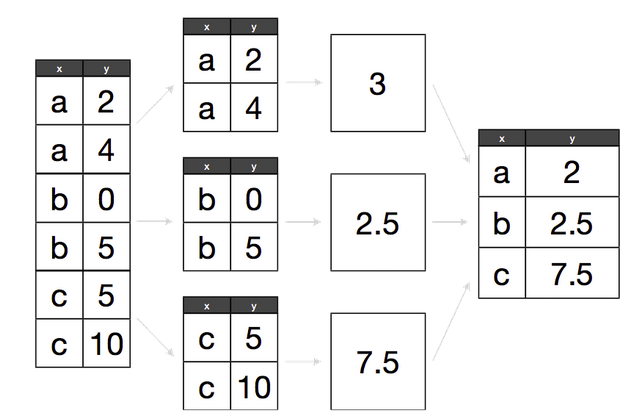
\includegraphics[width=0.75\textwidth]{../img/01_s-a-c.png}
    \caption{Ejemplificación del split-apply-combine \textcite[Split-Apply-Combine]{vaidyanathan2014r}.}
    \label{fig:sac}
\end{figure}

Entendamos mejor:

\begin{Shaded}
\begin{Highlighting}[]
\NormalTok{letras <-}\StringTok{ }\KeywordTok{sample}\NormalTok{(letters, }\DecValTok{3}\NormalTok{)}
\NormalTok{df <-}\StringTok{ }\KeywordTok{data.frame}\NormalTok{(}
  \DataTypeTok{letra =} \NormalTok{letras[}\KeywordTok{rep}\NormalTok{(}\KeywordTok{seq}\NormalTok{(letras), }\DecValTok{4}\NormalTok{)],}
  \DataTypeTok{valor =} \KeywordTok{sample}\NormalTok{(}\DecValTok{1}\NormalTok{:}\DecValTok{10}\NormalTok{, }\DataTypeTok{size =} \DecValTok{12}\NormalTok{, }\DataTypeTok{replace =} \NormalTok{T)}
\NormalTok{)}
\NormalTok{df <-}\StringTok{ }\NormalTok{df[}\KeywordTok{order}\NormalTok{(df$letra), ]}
\NormalTok{df}
\end{Highlighting}
\end{Shaded}

\begin{verbatim}
##    letra valor
## 3      h     5
## 6      h     5
## 9      h     4
## 12     h     9
## 1      j     5
## 4      j    10
## 7      j     3
## 10     j     6
## 2      w     5
## 5      w     2
## 8      w     2
## 11     w     7
\end{verbatim}

Queremos estimar la media del valor para cada tipo de letra.

\begin{Shaded}
\begin{Highlighting}[]
\CommentTok{# Dividimos}
\NormalTok{for (l in }\KeywordTok{unique}\NormalTok{(df$letra) )\{}
  \KeywordTok{print}\NormalTok{(df[l ==}\StringTok{ }\NormalTok{df$letra, ])}
\NormalTok{\}}
\end{Highlighting}
\end{Shaded}

\begin{verbatim}
##    letra valor
## 3      h     5
## 6      h     5
## 9      h     4
## 12     h     9
##    letra valor
## 1      j     5
## 4      j    10
## 7      j     3
## 10     j     6
##    letra valor
## 2      w     5
## 5      w     2
## 8      w     2
## 11     w     7
\end{verbatim}

\begin{Shaded}
\begin{Highlighting}[]
\CommentTok{# Aplicamos}
\NormalTok{for (l in }\KeywordTok{unique}\NormalTok{(df$letra) )\{}
  \KeywordTok{print}\NormalTok{(}\KeywordTok{mean}\NormalTok{(df[l ==}\StringTok{ }\NormalTok{df$letra, ]$valor))}
\NormalTok{\}}
\end{Highlighting}
\end{Shaded}

\begin{verbatim}
## [1] 5.75
## [1] 6
## [1] 4
\end{verbatim}

\begin{Shaded}
\begin{Highlighting}[]
\CommentTok{# Combinamos}
\NormalTok{medias <-}\StringTok{ }\KeywordTok{list}\NormalTok{()}
\NormalTok{for (l in }\KeywordTok{unique}\NormalTok{(df$letra) )\{}
  \NormalTok{medias[[l]] <-}\StringTok{ }\KeywordTok{mean}\NormalTok{(df[l ==}\StringTok{ }\NormalTok{df$letra, ]$valor)}
\NormalTok{\}}
\KeywordTok{as.data.frame}\NormalTok{(}\KeywordTok{list}\NormalTok{(}\DataTypeTok{letras =} \KeywordTok{names}\NormalTok{(medias), }\DataTypeTok{medias =} \KeywordTok{unname}\NormalTok{(}\KeywordTok{unlist}\NormalTok{(medias))))}
\end{Highlighting}
\end{Shaded}

\begin{verbatim}
##   letras medias
## 1      h   5.75
## 2      j   6.00
## 3      w   4.00
\end{verbatim}

R tiene muchas funciones que facilitan realizar este tipo de
operaciones. En particular, la familia \texttt{apply} fue pensada para
realizar ese tipo de operaciones.

\subsection{apply}\label{apply}

\texttt{apply} aplica una función a cada fila o columna en una matriz.

\begin{Shaded}
\begin{Highlighting}[]
\NormalTok{m <-}\StringTok{ }\KeywordTok{matrix}\NormalTok{(}\KeywordTok{c}\NormalTok{(}\DecValTok{1}\NormalTok{:}\DecValTok{5}\NormalTok{, }\DecValTok{6}\NormalTok{:}\DecValTok{10}\NormalTok{), }\DataTypeTok{nrow =} \DecValTok{5}\NormalTok{, }\DataTypeTok{ncol =} \DecValTok{2}\NormalTok{)}
\CommentTok{# 1 is the row index 2 is the column index}
\NormalTok{m}
\end{Highlighting}
\end{Shaded}

\begin{verbatim}
##      [,1] [,2]
## [1,]    1    6
## [2,]    2    7
## [3,]    3    8
## [4,]    4    9
## [5,]    5   10
\end{verbatim}

\begin{Shaded}
\begin{Highlighting}[]
\KeywordTok{apply}\NormalTok{(m, }\DecValTok{1}\NormalTok{, sum)}
\end{Highlighting}
\end{Shaded}

\begin{verbatim}
## [1]  7  9 11 13 15
\end{verbatim}

\begin{Shaded}
\begin{Highlighting}[]
\KeywordTok{apply}\NormalTok{(m, }\DecValTok{2}\NormalTok{, sum)}
\end{Highlighting}
\end{Shaded}

\begin{verbatim}
## [1] 15 40
\end{verbatim}

\textbf{Ejercicio} Haz una función que reciba un vector y devuelva la
suma de la posición $v_i + v_{i + 1}$. Para el n-esimo elemento, suma el
primero. Aplica esa función a las columnas y filas de la matriz m.

\subsection{lapply}\label{lapply}

\texttt{lapply} aplica una función a cada elemento en una lista. Como
sabemos, un \texttt{data.frame} es únicamente un estilo particular de
lista tal que todos sus elementos tienen el mismo tamaño. Por ende,
también podemos utilizar \texttt{lapply} para iterar sobre las columnas
de un \texttt{data.frame}.

\begin{Shaded}
\begin{Highlighting}[]
\NormalTok{lista <-}\StringTok{ }\KeywordTok{list}\NormalTok{(}\DataTypeTok{a =} \DecValTok{1}\NormalTok{:}\DecValTok{10}\NormalTok{, }\DataTypeTok{b =} \DecValTok{2}\NormalTok{:}\DecValTok{20}\NormalTok{)}
\KeywordTok{lapply}\NormalTok{(lista, mean)}
\end{Highlighting}
\end{Shaded}

\begin{verbatim}
## $a
## [1] 5.5
## 
## $b
## [1] 11
\end{verbatim}

\begin{Shaded}
\begin{Highlighting}[]
\NormalTok{df <-}\StringTok{ }\KeywordTok{data.frame}\NormalTok{(}\DataTypeTok{a =} \DecValTok{1}\NormalTok{:}\DecValTok{10}\NormalTok{, }\DataTypeTok{b =} \DecValTok{11}\NormalTok{:}\DecValTok{20}\NormalTok{)}
\KeywordTok{lapply}\NormalTok{(df, mean)}
\end{Highlighting}
\end{Shaded}

\begin{verbatim}
## $a
## [1] 5.5
## 
## $b
## [1] 15.5
\end{verbatim}

El \texttt{summary} de un data.frame genera un resumen para los vectores
que la conforman de acuerdo a la clase de la misma. Genera una función
que regrese una tabla de frecuencias para factores y caracteres o una
lista con media, desviación estándar para vectores numéricos o enteros.
Aplícalo a la base diamonds usando lapply.

\subsection{sapply}\label{sapply}

\texttt{sapply} es otra versión de \texttt{lapply} que regresa una lista
de una matriz cuando es apropiado.

\begin{Shaded}
\begin{Highlighting}[]
\NormalTok{x <-}\StringTok{ }\KeywordTok{sapply}\NormalTok{(lista, mean, }\DataTypeTok{simplify =} \NormalTok{F)}
\NormalTok{x}
\end{Highlighting}
\end{Shaded}

\begin{verbatim}
## $a
## [1] 5.5
## 
## $b
## [1] 11
\end{verbatim}

\begin{Shaded}
\begin{Highlighting}[]
\NormalTok{x <-}\StringTok{ }\KeywordTok{sapply}\NormalTok{(lista, mean, }\DataTypeTok{simplify =} \NormalTok{T)}
\NormalTok{x}
\end{Highlighting}
\end{Shaded}

\begin{verbatim}
##    a    b 
##  5.5 11.0
\end{verbatim}

\textbf{Ejercicio} Obtén un vector tipo caracter con los nombres de las
clases de las columnas de iris.

\textbf{Ejercicio} Repite el ejercicio de la suma rara pero usa
\texttt{sapply}.

\emph{Recuerda la instrucción}: Haz una función que reciba un vector y
devuelva la suma de la posición $v_i + v_{i + 1}$. Para el n-esimo
elemento, suma el primero. Utiliza \texttt{sapply} para realizar esta
operacion.

\subsection{mapply}\label{mapply}

\texttt{mapply} es como la versión multivariada de \texttt{sapply}. Le
aplica una función a todos los elementos correspondientes de un
argumento.

\begin{Shaded}
\begin{Highlighting}[]
\NormalTok{l1 <-}\KeywordTok{list}\NormalTok{(}\DataTypeTok{a =} \KeywordTok{c}\NormalTok{(}\DecValTok{1}\NormalTok{:}\DecValTok{5}\NormalTok{), }\DataTypeTok{b =} \KeywordTok{c}\NormalTok{(}\DecValTok{6}\NormalTok{:}\DecValTok{10}\NormalTok{))}
\NormalTok{l2 <-}\StringTok{ }\KeywordTok{list}\NormalTok{(}\DataTypeTok{c =} \KeywordTok{c}\NormalTok{(}\DecValTok{11}\NormalTok{:}\DecValTok{15}\NormalTok{), }\DataTypeTok{d =} \KeywordTok{c}\NormalTok{(}\DecValTok{16}\NormalTok{:}\DecValTok{20}\NormalTok{))}
\NormalTok{l1}
\end{Highlighting}
\end{Shaded}

\begin{verbatim}
## $a
## [1] 1 2 3 4 5
## 
## $b
## [1]  6  7  8  9 10
\end{verbatim}

\begin{Shaded}
\begin{Highlighting}[]
\NormalTok{l2}
\end{Highlighting}
\end{Shaded}

\begin{verbatim}
## $c
## [1] 11 12 13 14 15
## 
## $d
## [1] 16 17 18 19 20
\end{verbatim}

\begin{Shaded}
\begin{Highlighting}[]
\KeywordTok{mapply}\NormalTok{(sum, l1$a, l1$b, l2$c, l2$d)}
\end{Highlighting}
\end{Shaded}

\begin{verbatim}
## [1] 34 38 42 46 50
\end{verbatim}

\begin{Shaded}
\begin{Highlighting}[]
\NormalTok{l1[[}\StringTok{"a"}\NormalTok{]][}\DecValTok{1}\NormalTok{] +}\StringTok{ }\NormalTok{l1[[}\StringTok{"b"}\NormalTok{]][}\DecValTok{1}\NormalTok{] +}\StringTok{ }\NormalTok{l2[[}\StringTok{"c"}\NormalTok{]][}\DecValTok{1}\NormalTok{] +}\StringTok{ }\NormalTok{l2[[}\StringTok{"d"}\NormalTok{]][}\DecValTok{1}\NormalTok{]}
\end{Highlighting}
\end{Shaded}

\begin{verbatim}
## [1] 34
\end{verbatim}

\subsection{tapply}\label{tapply}

\texttt{tapply} le aplica una función a subconjuntos de un vector.

\begin{Shaded}
\begin{Highlighting}[]
\KeywordTok{head}\NormalTok{(warpbreaks)}
\end{Highlighting}
\end{Shaded}

\begin{verbatim}
##   breaks wool tension
## 1     26    A       L
## 2     30    A       L
## 3     54    A       L
## 4     25    A       L
## 5     70    A       L
## 6     52    A       L
\end{verbatim}

\begin{Shaded}
\begin{Highlighting}[]
\KeywordTok{with}\NormalTok{(warpbreaks, }\KeywordTok{tapply}\NormalTok{(breaks, }\KeywordTok{list}\NormalTok{(wool, tension), mean))}
\end{Highlighting}
\end{Shaded}

\begin{verbatim}
##          L        M        H
## A 44.55556 24.00000 24.55556
## B 28.22222 28.77778 18.77778
\end{verbatim}

\begin{Shaded}
\begin{Highlighting}[]
\KeywordTok{tapply}\NormalTok{(warpbreaks$breaks, }
       \KeywordTok{list}\NormalTok{(}\DataTypeTok{wool =} \NormalTok{warpbreaks$wool, }\DataTypeTok{tension =} \NormalTok{warpbreaks$tension), }
       \NormalTok{mean)}
\end{Highlighting}
\end{Shaded}

\begin{verbatim}
##     tension
## wool        L        M        H
##    A 44.55556 24.00000 24.55556
##    B 28.22222 28.77778 18.77778
\end{verbatim}

\textbf{Ejercicio}

\subsection{by}\label{by}

\texttt{by} le aplica una función a subconjuntos de un
\texttt{data.frame}. Se divide un data.frame según los valores de de uno
o más factores. Se aplica la función FUN a cada subconjunto.

\begin{Shaded}
\begin{Highlighting}[]
\KeywordTok{head}\NormalTok{(iris)}
\end{Highlighting}
\end{Shaded}

\begin{verbatim}
##   Sepal.Length Sepal.Width Petal.Length Petal.Width Species
## 1          5.1         3.5          1.4         0.2  setosa
## 2          4.9         3.0          1.4         0.2  setosa
## 3          4.7         3.2          1.3         0.2  setosa
## 4          4.6         3.1          1.5         0.2  setosa
## 5          5.0         3.6          1.4         0.2  setosa
## 6          5.4         3.9          1.7         0.4  setosa
\end{verbatim}

\begin{Shaded}
\begin{Highlighting}[]
\KeywordTok{by}\NormalTok{(}\DataTypeTok{data =} \NormalTok{iris[, }\DecValTok{1}\NormalTok{:}\DecValTok{2}\NormalTok{], }\DataTypeTok{INDICES =} \NormalTok{iris[, }\StringTok{"Species"}\NormalTok{], }\DataTypeTok{FUN =} \NormalTok{summary)}
\end{Highlighting}
\end{Shaded}

\begin{verbatim}
## iris[, "Species"]: setosa
##   Sepal.Length    Sepal.Width   
##  Min.   :4.300   Min.   :2.300  
##  1st Qu.:4.800   1st Qu.:3.200  
##  Median :5.000   Median :3.400  
##  Mean   :5.006   Mean   :3.428  
##  3rd Qu.:5.200   3rd Qu.:3.675  
##  Max.   :5.800   Max.   :4.400  
## -------------------------------------------------------- 
## iris[, "Species"]: versicolor
##   Sepal.Length    Sepal.Width   
##  Min.   :4.900   Min.   :2.000  
##  1st Qu.:5.600   1st Qu.:2.525  
##  Median :5.900   Median :2.800  
##  Mean   :5.936   Mean   :2.770  
##  3rd Qu.:6.300   3rd Qu.:3.000  
##  Max.   :7.000   Max.   :3.400  
## -------------------------------------------------------- 
## iris[, "Species"]: virginica
##   Sepal.Length    Sepal.Width   
##  Min.   :4.900   Min.   :2.200  
##  1st Qu.:6.225   1st Qu.:2.800  
##  Median :6.500   Median :3.000  
##  Mean   :6.588   Mean   :2.974  
##  3rd Qu.:6.900   3rd Qu.:3.175  
##  Max.   :7.900   Max.   :3.800
\end{verbatim}

Puedo calcular, por ejemplo, la suma de los valores del largo y ancho de
los sépalos en la base de datos iris según la especie.

\begin{Shaded}
\begin{Highlighting}[]
\NormalTok{res <-}\StringTok{ }\KeywordTok{by}\NormalTok{(iris[, }\KeywordTok{c}\NormalTok{(}\StringTok{"Sepal.Length"}\NormalTok{, }\StringTok{"Sepal.Width"}\NormalTok{)], iris[, }\StringTok{"Species"}\NormalTok{], sum)}
\end{Highlighting}
\end{Shaded}

Posteriormente, se pueden combinar los elementos.

\begin{Shaded}
\begin{Highlighting}[]
\KeywordTok{as.data.frame}\NormalTok{(}\KeywordTok{list}\NormalTok{(}
  \StringTok{"species"} \NormalTok{=}\StringTok{ }\KeywordTok{names}\NormalTok{(res), }
  \StringTok{"suma"} \NormalTok{=}\StringTok{ }\KeywordTok{sapply}\NormalTok{(}\KeywordTok{seq}\NormalTok{(}\KeywordTok{length}\NormalTok{(res)), }\DataTypeTok{FUN =} \NormalTok{function(i) res[[i]])}
  \NormalTok{))}
\end{Highlighting}
\end{Shaded}

\begin{verbatim}
##      species  suma
## 1     setosa 421.7
## 2 versicolor 435.3
## 3  virginica 478.1
\end{verbatim}

\textbf{Ejercicio} Vuelve a utilizar la base de diamonds para calcular
el promedio de carat según cut y color.

\begin{verbatim}
##   carat       cut color clarity depth table price    x    y    z
## 1  0.23     Ideal     E     SI2  61.5    55   326 3.95 3.98 2.43
## 2  0.21   Premium     E     SI1  59.8    61   326 3.89 3.84 2.31
## 3  0.23      Good     E     VS1  56.9    65   327 4.05 4.07 2.31
## 4  0.29   Premium     I     VS2  62.4    58   334 4.20 4.23 2.63
## 5  0.31      Good     J     SI2  63.3    58   335 4.34 4.35 2.75
## 6  0.24 Very Good     J    VVS2  62.8    57   336 3.94 3.96 2.48
\end{verbatim}

\subsection{replicate}\label{replicate}

\texttt{replicate} es una función muy útil sobretodo en el contexto de
simulación.

\begin{Shaded}
\begin{Highlighting}[]
\KeywordTok{replicate}\NormalTok{(}\DecValTok{5}\NormalTok{, }\KeywordTok{rnorm}\NormalTok{(}\DecValTok{6}\NormalTok{), }\DataTypeTok{simplify =} \NormalTok{F)}
\end{Highlighting}
\end{Shaded}

\begin{verbatim}
## [[1]]
## [1] -1.48174362  0.66978164 -0.78426278 -0.45197092  1.02655102  0.02008344
## 
## [[2]]
## [1] -0.5126506 -0.4285076  0.5632417  0.1028410  0.1923036  1.1650204
## 
## [[3]]
## [1] -0.18038327  0.33794788  0.08232277 -0.10389078 -1.14011737 -0.61650967
## 
## [[4]]
## [1]  0.7039886 -2.2066521 -0.8376586  1.7216593  0.4360063  0.7571990
## 
## [[5]]
## [1]  1.5398858  1.5393945  2.1829996 -0.9953758 -0.3013422  0.6005107
\end{verbatim}

\begin{Shaded}
\begin{Highlighting}[]
\KeywordTok{replicate}\NormalTok{(}\DecValTok{6}\NormalTok{, }\KeywordTok{rnorm}\NormalTok{(}\DecValTok{4}\NormalTok{), }\DataTypeTok{simplify =} \NormalTok{T)}
\end{Highlighting}
\end{Shaded}

\begin{verbatim}
##            [,1]       [,2]       [,3]       [,4]      [,5]       [,6]
## [1,] -0.3633049  0.8675148 -1.3168208  1.5543102 0.6130339  0.5737528
## [2,] -0.2211350 -0.1700282 -0.6075526  0.3306465 0.7158021  0.2225771
## [3,] -0.1981113  1.1900491 -0.9454914  0.2031200 0.6501763  1.1414076
## [4,]  0.6676305  0.9188715  1.2493954 -2.5829970 0.7201334 -0.6722725
\end{verbatim}

\begin{Shaded}
\begin{Highlighting}[]
\KeywordTok{hist}\NormalTok{(}\KeywordTok{replicate}\NormalTok{(}\DecValTok{100}\NormalTok{, }\KeywordTok{mean}\NormalTok{(}\KeywordTok{rexp}\NormalTok{(}\DecValTok{10}\NormalTok{))))}
\end{Highlighting}
\end{Shaded}

\begin{figure}[htbp]
\centering
\includegraphics{2_basico_files/figure-latex/unnamed-chunk-47-1.pdf}
\end{figure}

\textbf{Ejercicio} Replica el ejercicio de muestras bootstrap utilizando
replicate.

Recordando:

\begin{enumerate}
\item Genera un vector x de tamaño 1000 con realizaciones de una normal media 10, varianza 3. 
\item Crea 100 muestras bootstrap del vector x.
\item Calcula la media para cada una de tus muestras.
\item Grafica con la función hist() el vector de medias de tus muestras.
\end{enumerate}

\subsection{¿Puede ser más fácil?}\label{puede-ser-mas-facil}

La familia \texttt{apply} viene con R básico. Sin embargo, hay 3
implementaciones excelentes del paradigma split-apply-combine:
\texttt{plyr}, \texttt{dplyr} y \texttt{data.table}.

Si la familia apply es poderosa, se queda corta comparada con estos
tres. \texttt{plyr} es la primera versión de s-a-c de Wickham.
Posteriormente, mejoró muchas de las funciones en \texttt{dplyr}
sobretodo entorno a velocidad y facilidad de uso. \texttt{plyr} no
termina de ser relevante pues varias de sus funciones aun no están en
\texttt{dplyr}.

\texttt{data.table}, es una implementación con una tradición muy
diferente y tiene también funciones muy poderosas aunque con una
sintaxis muy distinta a \texttt{dplyr}. Es absurdamente eficiente y
tiene múltiples aplicaciones.

Muchas de las funciones en \texttt{dplyr} también están implementadas en
\texttt{data.table}. Cuál usar es cuestión de gustos. Depende de con qué
se acomoda cada quién pero, para algunas cosas uno es superior al otro y
viceversa.

\printbibliography

\begin{Shaded}
\begin{Highlighting}[]
\KeywordTok{sessionInfo}\NormalTok{()}
\end{Highlighting}
\end{Shaded}

\begin{verbatim}
## R version 3.2.2 (2015-08-14)
## Platform: x86_64-pc-linux-gnu (64-bit)
## Running under: Ubuntu 15.04
## 
## locale:
##  [1] LC_CTYPE=en_US.UTF-8       LC_NUMERIC=C              
##  [3] LC_TIME=es_MX.UTF-8        LC_COLLATE=en_US.UTF-8    
##  [5] LC_MONETARY=es_MX.UTF-8    LC_MESSAGES=en_US.UTF-8   
##  [7] LC_PAPER=es_MX.UTF-8       LC_NAME=C                 
##  [9] LC_ADDRESS=C               LC_TELEPHONE=C            
## [11] LC_MEASUREMENT=es_MX.UTF-8 LC_IDENTIFICATION=C       
## 
## attached base packages:
## [1] stats     graphics  grDevices utils     datasets  base     
## 
## other attached packages:
## [1] ggplot2_2.0.0   xtable_1.7-4    rformat_0.1     rmarkdown_0.8.1
## 
## loaded via a namespace (and not attached):
##  [1] Rcpp_0.12.2.2    digest_0.6.8     plyr_1.8.3       grid_3.2.2      
##  [5] gtable_0.1.2     formatR_1.2.1    magrittr_1.5     evaluate_0.8    
##  [9] scales_0.3.0     stringi_1.0-1    tools_3.2.2      stringr_1.0.0   
## [13] munsell_0.4.2    yaml_2.1.13      colorspace_1.2-6 htmltools_0.2.6 
## [17] knitr_1.11       methods_3.2.2
\end{verbatim}

\end{document}
